\documentclass[11pt,twocolumn]{article}
\usepackage{naaclhlt2013}
\usepackage{inconsolata}
\usepackage{helvet}
\usepackage{mathptmx}
\usepackage{microtype}

\usepackage{amsmath}
\usepackage{flafter}
\usepackage{graphicx}
\usepackage{multirow}
\usepackage[section]{placeins}
\usepackage{setspace}
\usepackage{rotating}

\begin{document}
\title{PyMEANT: Automatic Semantic MT Evaluation in Python}
\author{
    Roger Que\\
    {\tt query@jhu.edu}\\
    {\tt https://github.com/query/mt-submissions/tree/master/project}
}
\maketitle


\begin{abstract}
In this paper, I present PyMEANT, a Python implementation of the MEANT
machine translation evaluation metric \cite{Lo:2012}.
MEANT matches semantic frames and arguments, as identified by a shallow
semantic parse, in order to ensure the preservation of each sentence's
argument structure.
The semantic similarity of word pairs is judged by the Jaccard index of
their respective sets of co-occurring contexts.
Tests show that PyMEANT achieves better pairwise ranking accuracy
against human adequacy judgments than BLEU.
\end{abstract}


\section{Introduction}

It is generally accepted that human judgments of translation adequacy
are ultimately based on the semantic content of a hypothesis.
Therefore, an automatic evaluation process that successfully
incorporates semantic information should, in theory, obtain better
correlation with human judgments than a semantically-ignorant evaluator
run on the same data.

Currently, most widely used translation quality metrics are based
primarily on measures of $n$-gram precision and recall, including
BLEU \cite{Papineni:2002} and METEOR \cite{Banerjee:2005}.
This approach has the advantage of being easy to incorporate into
translation systems due to its relatively inexpensive scoring method,
and does a good job of capturing translation fluency.
However, it also fails to sufficiently capture important aspects of a
sentence's meaning.
With BLEU, in particular, a hypothesis' phrases may be permuted around
bigram mismatch sites to yield a second hypothesis that is clearly
incoherent, yet still has the same score \cite{Callison-Burch:2006}.
This presents a problem for evaluation not only on fluency, but on
adequacy as well.
The implication is that, in many cases, a sentence's arguments may be
reordered in a way that preserves its BLEU score, but completely changes
its meaning.
It is clear that $n$-gram measurements alone are not sufficient to
ensure that important semantic relations are kept intact, and that
more direct inspection of a hypothesis' semantic content is needed.

However, semantic evaluation is a difficult problem for a number of
reasons.
Foremost among these issues is the question of how to capture semantic
information in a usefully comparable way, so that translation hypotheses
may be checked against their respective references.
Although proposals for the representation of deep semantic structure,
such as AMR's acyclic graphical notation \cite{Banarescu:2013}, and
corresponding parsers into these representations \cite{Flanigan:2014}
exist, the best method for measuring the similarity of multiple
instances of these complex structures is still an open question.
Conceptually straightforward methods, such as graph edit distance, are
NP-hard and thus present computational tractability problems.
Ideally, we would like a metric with relatively low overhead that
avoids constructing large graphs or other complex structures to
represent each sentence.


\section{The MEANT metric}

In order to avoid these technical challenges, MEANT takes a simplified
approach to the incorporation of semantic information.
Instead of attempting to discern the full semantic structure of a
sentence, it performs a shallow semantic parse that identifies a series
of frames containing verbs, also referred to as \textit{predicates}, and
their semantic role arguments.
It then aligns frames with similar predicates together, and computes
the total similarity of the predicates and arguments in order to yield
a final score.


\subsection{Semantic frame identification}

The first task in MEANT is the extraction of frames from raw sentences,
which is equivalent to a semantic role labeling task.
There are several SRL tagging schemata in wide use, chief among them
FrameNet \cite{Fillmore:2003} and PropBank \cite{Palmer:2005}.
These two systems differ primarily in their approach to generalizing
over semantic roles from verb to verb.

FrameNet attempts to define generic roles, such as \textsf{Addressee}
and \textsf{Seller}, than can be applied to multiple verbs.
This introduces the possibility of weighting arguments based on their
role class.
For example, with sentences that describe a commercial transaction, we
may choose to emphasize the parties involved over the goods exchanged by
weighting the former more heavily.
However, this also makes the construction of a corpus more difficult,
as argument classes must remain consistent over all verbs to which they
apply.

PropBank, on the other hand, defines arguments on a verb-by-verb basis,
and only informally correlates them across different verbs.
For this reason, although \textsf{Arg0} is usually a prototypical
agent, and \textsf{Arg1} is often a patient or theme, it is improper to
construe instances of these arguments attached to specific verbs as part
of a broader argument class.

PyMEANT uses the PropBank tagging scheme, following the lead of the
original MEANT implementation.
The ASSERT automatic semantic role tagger \cite{Pradhan:2004} is used to
identify individual frames.
The predicates of frames identified by ASSERT for a sample translation
hypothesis and its corresponding reference are shown in
Figure~\ref{fig:predicates}.

\begin{figure}
\begin{doublespacing}
\begin{description}
\item \textbf{MTO:}
When the reporter $\underset{\textrm{1}}{\underline{\textrm{went}}}$ to
the hotel at 4:00 p.m., however, most of the job-seekers to
$\underset{\textrm{2}}{\underline{\textrm{participate}}}$ in the
recruitment, not many people will
$\underset{\textrm{3}}{\underline{\textrm{come}}}$ back, but has been
can $\underset{\textrm{4}}{\underline{\textrm{tell}}}$ all days of the
South China Sea north of accent.

\item \textbf{REF:}
It was four in the afternoon when our reporter
$\underset{\textrm{A}}{\underline{\textrm{arrived}}}$ at the hostel, but
most of the job-seekers were still elsewhere
$\underset{\textrm{B}}{\underline{\textrm{taking}}}$ part in job fairs
and not many had $\underset{\textrm{C}}{\underline{\textrm{returned}}}$
$\underset{\textrm{D}}{\underline{\textrm{yet}}}$.
However, one could already
$\underset{\textrm{E}}{\underline{\textrm{hear}}}$ accents from all over
the country.
\end{description}
\end{doublespacing}
\caption{\label{fig:predicates}
Semantic frame predicates identified by \mbox{ASSERT} for sample machine
translation output (MTO) and corresponding reference (REF) from the
DARPA GALE corpus.
}
\end{figure}


\subsection{\label{sec:lexsim} Lexical similarity measures}

Having identified the relevant predicates and arguments, we would now
like to determine how similar they are.
Ideally, the measure we use should be able to capture some intuitions
about the environments in which semantically related words occur.
As mentioned earlier, $n$-gram metrics such as BLEU and METEOR are
unlikely to be helpful here, particularly because of the short length
of the word strings involved.

MEANT relies on the notion that words with similar meaning are likely to
appear surrounded by similar contexts, and thus the set of words that
they co-occur with should strongly overlap.
There are several information-theoretic metrics for this type of
\textit{lexical similarity}.
PyMEANT uses the Jaccard similarity, which has been shown to be an
effective measure for use in MEANT \cite{Tumuluru:2012}, and is fairly
straightforward to implement.
Generally defined, for two sets $A$ and $B$, the Jaccard similarity is
the cardinality of their intersection divided by the cardinality of
their union:
\[
J(x,y)=\frac{\left|A\cap B\right|}{\left|A\cup B\right|}
\]

For our purposes, $A$ and $B$ are multisets containing the word types
with which some word types $a$ and $b$ have co-occurred.
We use a co-occurrence window size to restrict the number of possible
pairs.
PyMEANT's default window size is 3, meaning that two words must occur
together within a single 3-word span to be considered co-occurring;
equivalently, they may be separated by at most one other word.
Sizes up to 13 have been tested,
though these longer windows yield no corresponding increase in MEANT's
overall accuracy \cite{Tumuluru:2012}.
Defined, then, in terms of the number of co-occurrences $c(a,b)$ for
the words $a$ and $b$, and the set of all word types $W$, the Jaccard
similarity coefficient $J(a,b)$ is:
\[
J(x,y)=\frac{\sum_{w\in W}\min(c(a,w),\,c(b,w))}
            {\sum_{w\in W}\max(c(a,w),\,c(b,w))}
\]


\subsection{Predicate and argument matching}

We now turn to computation of the overall MEANT score.
This is accomplished by aligning semantic frames between the hypothesis
and the reference, then the words in each of the frames' arguments, and
summing over the lexical similarity of each pair of aligned words.

MEANT aligns individual words with each other by performing maximum
bipartite matching over a graph with each node representing a single
word.
Edges connect each hypothesis node with each reference node, weighted
by the lexical similarity of the two words at each end.
After matching, each word is aligned to exactly zero or one words on the
opposite side of the graph.
This process is first used to align frames with each other, using their
predicates as the graph nodes.
Then, for each pair of frames, the words of arguments with the same
label are also aligned to each other, using the words themselves as
nodes.
A sample predicate alignment graph is illustrated in
Figure~\ref{fig:alignment}, with the weights used for matching shown in
Table~\ref{tab:similarity}.

\begin{figure}
\center
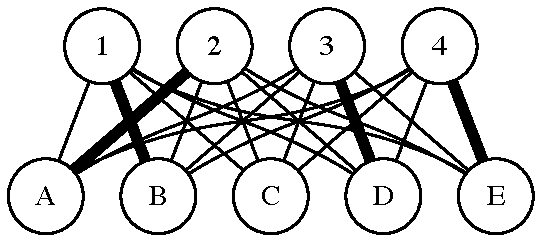
\includegraphics[scale=0.75]{predicate-alignment}
\caption{\label{fig:alignment}
A bipartite graph representation of the possible alignments of the
predicates shown in Figure~\ref{fig:predicates}.
Thick lines indicate the alignments selected by the bipartite matching
algorithm.
}
\end{figure}

\begin{table}
\center
\begin{tabular}{ll|rrrrr}
&
&
\multicolumn{4}{|c}{\textbf{MT output}} \\
&
&
\multicolumn{1}{c}{\textbf{1}} &
\multicolumn{1}{c}{\textbf{2}} &
\multicolumn{1}{c}{\textbf{3}} &
\multicolumn{1}{c}{\textbf{4}} \\
\hline
\multirow{5}{*}{\begin{sideways}\textbf{Reference}\end{sideways}} &
\textbf{A} &
0.117 &
\textbf{0.130} &
0.090 &
0.121 \\
&
\textbf{B} &
\textbf{0.194} &
0.085 &
0.166 &
0.165 \\
&
\textbf{C} &
0.165 &
0.119 &
0.122 &
0.194 \\
&
\textbf{D} &
0.208 &
0.067 &
\textbf{0.238} &
0.196 \\
&
\textbf{E} &
0.146 &
0.127 &
0.142 &
\textbf{0.301}
\end{tabular}
\caption{\label{tab:similarity}
Pairwise Jaccard similarity scores for the predicates shown in
Figure~\ref{fig:predicates}.
The alignments selected by the bipartite matching algorithm are
highlighted in bold.
}
\end{table}

The similarity score for each predicate and argument is computed by
summing over the Jaccard coefficient for each pair of aligned words,
then dividing by word length of either the hypothesis or the reference
side, whichever is longer.
In algebraic terms, for some word vector $\vec h$ representing a
predicate or argument in the hypothesis, the corresponding
reference-side vector $\vec r$, and a set of alignments $A(\vec h, \vec
r)$ containing ordered alignment word pairs $(i,j)$, the similarity
score $S(\vec h, \vec r)$ is defined as:
\[
S(\vec h, \vec r)=\frac{\sum_{(w,x)\in A(\vec h,\vec r)} J(w,x)}
                       {\max(|\vec h|, |\vec r|)}
\]

We now compute a total score for the entire sentence.
The score for each frame is weighted by the fraction of words it covers
in the overall sentence, such that larger, and thus more semantically
important, frames have more influence over the final score than smaller
ones.
A frame $\mathbf{f}$'s coverage ratio in a sentence $V$, denoted
$v(\mathbf{f},V)$, is equal to:
\[
v(\mathbf{f},V) = \frac{|\mathbf{f}|}{|V|}
\]

For each hypothesis $H$ and reference $R$, separate precision and recall
scores $p(H,R)$ and $r(H,R)$ are first computed.
The precision is normalized against the maximum possible score given
total coverage of the frames in the MT output, while the recall is
normalized against the same for the reference.
Let $n(\textbf{f})$ denote the number of arguments to frame
$\textbf{f}$, including the predicate; let $A(H,R)$ denote the set of
frame alignments $(\textbf{f},\textbf{g})$ between the sentences $H$ and
$R$; and let $A(\textbf{f},\textbf{g})$ denote the set of argument
alignments $(\vec h,\vec r)$ between frames $\textbf{f}$ and
$\textbf{g}$.
Then the precision and recall are:
\begin{align*}
p(H,R)&=&\hspace{-10pt}\sum_{(\textbf{f},\textbf{g})\in A(H,R)}
\left[
\frac{v(\textbf{f},V)}{n(\textbf{f})}\cdot
\sum_{(\vec h,\vec r)\in A(\textbf{f},\textbf{g})} S(\vec h,\vec r)
\right] \\
r(H,R)&=&\hspace{-10pt}\sum_{(\textbf{f},\textbf{g})\in A(H,R)}
\left[
\frac{v(\textbf{g},V)}{n(\textbf{g})}\cdot
\sum_{(\vec h,\vec r)\in A(\textbf{f},\textbf{g})} S(\vec h,\vec r)
\right]
\end{align*}

The final MEANT score is the $F_1$ measure:
\[
\textrm{MEANT}(H,R)=2\cdot\frac
{p(H,R)\cdot r(H,R)}
{p(H,R)+r(H,R)}
\]

Later revisions of MEANT add tunable parameters that control the
relative importance of predicates and argument classes \cite{Lo:2013}.
PyMEANT does not implement this feature, and so all predicates and
arguments are weighted equally in the final computation.


\section{Results}

PyMEANT was tested by measuring the total accuracy of pairwise
judgments on the DARPA GALE 2.5 broadcast news (BN) data sets for the
Arabic--English and Chinese--English language pairs.
For each translation segment, ``correct'' pairwise rankings between MT
systems were obtained by taking all pairs of systems and comparing the
mean human adequacy ratings.
The PyMEANT lexical similarity model was trained on the April 1995
section of Gigaword's \textit{New York Times} corpus;
due to the lack of tunable parameters for the evaluation metrics tested,
the data were not split into training and testing sets.

A comparison of correct pairwise judgments made by PyMEANT and 5-gram
per-sentence BLEU is shown in Table~\ref{tab:results}.
PyMEANT scores show higher correlation than BLEU on both tasks, with an
especially marked difference in performance on the Chinese--English
data.

\begin{table}
\center
\begin{tabular}{l|cc}
&
\textbf{ar--en} &
\textbf{zh--en} \\
\hline
\textbf{BLEU} &
37.74\% &
34.54\% \\
\textbf{PyMEANT} &
38.99\% &
41.18\%
\end{tabular}
\caption{\label{tab:results}
Correct pairwise rankings based on PyMEANT and 5-gram per-sentence BLEU
scores for the broadcast news language pairs in the DARPA GALE data set.
}
\end{table}


\section{Future work}

Although PyMEANT shows improved correlation with human judgments, this
comes at the expense of runtime and memory costs, in particular for
training the lexical similarity model and performing bipartite matching.
For arguments with many words, the $O(V^2 E)$ runtime of matching leads
to significant slowdowns.
Multiple system outputs can be scored in parallel to reduce runtime,
but even on a modern computer, PyMEANT took about 20 minutes to train a
lexical similarity model, then compute per-sentence scores for each of
the system outputs in the testing task.
BLEU scoring, on the other hand, was nearly instantaneous.

On the linguistic side, additional information may be obtainable from
the argument structure of noun phrases, which PropBank does not cover.
For example, the noun \textit{ovation} and the verb \textit{applaud}
point to the same concept, and so they can be expected to have similar
argument structure; however, the current PropBank-based parser would
not be able to capture this equivalence.
NomBank \cite{Meyers:2004} applies the PropBank model to nominal
constructions as well, which may improve MEANT's frame and argument
matching performance.


\begin{thebibliography}{}

\bibitem[\protect\citename{Banarescu \bgroup et al.\egroup
  }2013]{Banarescu:2013}
Laura Banarescu, Claire Bonial, Shu Cai, Madalina Georgescu, Kira Griffitt, Ulf
  Hermjakob, Kevin Knight, Philipp Koehn, Martha Palmer, and Nathan Schneider.
\newblock 2013.
\newblock Abstract meaning representation for sembanking.
\newblock In {\em Proceedings of the 7th Linguistic Annotation Workshop \&
  Interoperability with Discourse}, pages 178--186. Association for
  Computational Linguistics, August.

\bibitem[\protect\citename{Banerjee and Lavie}2005]{Banerjee:2005}
Satanjeev Banerjee and Alon Lavie.
\newblock 2005.
\newblock {METEOR}: An automatic metric for {MT} evaluation with improved
  correlation with human judgments.
\newblock In {\em Proceedings of the ACL Workshop on Intrinsic and Extrinsic
  Evaluation Measures for Machine Translation and/or Summarization}, pages
  65--72, Ann Arbor, Michigan, June. Association for Computational Linguistics.

\bibitem[\protect\citename{Callison-Burch \bgroup et al.\egroup
  }2006]{Callison-Burch:2006}
Chris Callison-Burch, Miles Osborne, and Philipp Koehn.
\newblock 2006.
\newblock Re-evaluating the role of {Bleu} in machine translation research.
\newblock In {\em In {EACL}}, pages 249--256.

\bibitem[\protect\citename{Fillmore \bgroup et al.\egroup }2003]{Fillmore:2003}
Charles~J. Fillmore, Christopher~R. Johnson, and Miriam~R.L. Petruck.
\newblock 2003.
\newblock Background to {FrameNet}.
\newblock {\em International journal of lexicography}, 16(3):235--250.

\bibitem[\protect\citename{Flanigan \bgroup et al.\egroup }2014]{Flanigan:2014}
Jeffrey Flanigan, Sam Thomson, Jaime Carbonell, Chris Dyer, and Noah~A. Smith.
\newblock 2014.
\newblock A discriminative graph-based parser for the {Abstract Meaning
  Representation}.
\newblock In {\em Proceedings of {ACL}}. Association for Computational
  Linguistics.

\bibitem[\protect\citename{Lo and Wu}2013]{Lo:2013}
Chi{-}kiu Lo and Dekai Wu.
\newblock 2013.
\newblock {MEANT} at {WMT} 2013: A tunable, accurate yet inexpensive semantic
  frame based {MT} evaluation metric.
\newblock In {\em Proceedings of the Eighth Workshop on Statistical Machine
  Translation}, pages 422--428. Association for Computational Linguistics.

\bibitem[\protect\citename{Lo \bgroup et al.\egroup }2012]{Lo:2012}
Chi{-}kiu Lo, Anand~Karthik Tumuluru, and Dekai Wu.
\newblock 2012.
\newblock Fully automatic semantic {MT} evaluation.
\newblock In {\em Proceedings of the 7th Workshop of Statistical Machine
  Translation}, pages 243--252. Association for Computational Linguistics.

\bibitem[\protect\citename{Meyers \bgroup et al.\egroup }2004]{Meyers:2004}
Adam Meyers, Ruth Reeves, Catherine Macleod, Rachel Szekely, Veronika
  Zielinska, Brian Young, and Ralph Grishman.
\newblock 2004.
\newblock The {NomBank} project: An interim report.
\newblock In {\em HLT-NAACL 2004 workshop: Frontiers in corpus annotation},
  pages 24--31.

\bibitem[\protect\citename{Palmer \bgroup et al.\egroup }2005]{Palmer:2005}
Martha Palmer, Daniel Gildea, and Paul Kingsbury.
\newblock 2005.
\newblock The proposition bank: An annotated corpus of semantic roles.
\newblock {\em Computational Linguistics}, 31(1):71--106.

\bibitem[\protect\citename{Papineni \bgroup et al.\egroup }2002]{Papineni:2002}
Kishore Papineni, Salim Roukos, Todd Ward, and Wei-Jing Zhu.
\newblock 2002.
\newblock Bleu: a method for automatic evaluation of machine translation.
\newblock In {\em Proceedings of the 40th Annual Meeting of the Association for
  Computational Linguistics}, pages 311--318, Philadelphia, Pennsylvania, USA,
  July. Association for Computational Linguistics.

\bibitem[\protect\citename{Pradhan \bgroup et al.\egroup }2004]{Pradhan:2004}
Sameer~S. Pradhan, Wayne Ward, Kadri Hacioglu, James~H. Martin, and Daniel
  Jurafsky.
\newblock 2004.
\newblock Shallow semantic parsing using support vector machines.
\newblock In {\em HLT-NAACL}, pages 233--240.

\bibitem[\protect\citename{Tumuluru \bgroup et al.\egroup }2012]{Tumuluru:2012}
Anand~Karthik Tumuluru, Chi{-}kiu Lo, and Dekai Wu.
\newblock 2012.
\newblock Accuracy and robustness in measuring the lexical similarity of
  semantic role fillers for automatic semantic {MT} evaluation.
\newblock In {\em 26th {Pacific} {Asia} Conference on Language, Information and
  Computation}, pages 574--581.

\end{thebibliography}

\end{document}
